\ssr{Приложение А}

ГОСТ 7.32-2017 (<<Отчёт о научно-исследовательской работе>>).


\includepdf[pages=-]{materials/2021-11gost_7.32-2017.pdf}

%<тут всякие слишком большие ништяки, которые вы хотели бы добавить в отчет>

\ssr{Приложение Б}

Инструкция по оформлению ВКР и проверке на объем заимствования для студентов МГТУ им. Н.Э. Баумана.

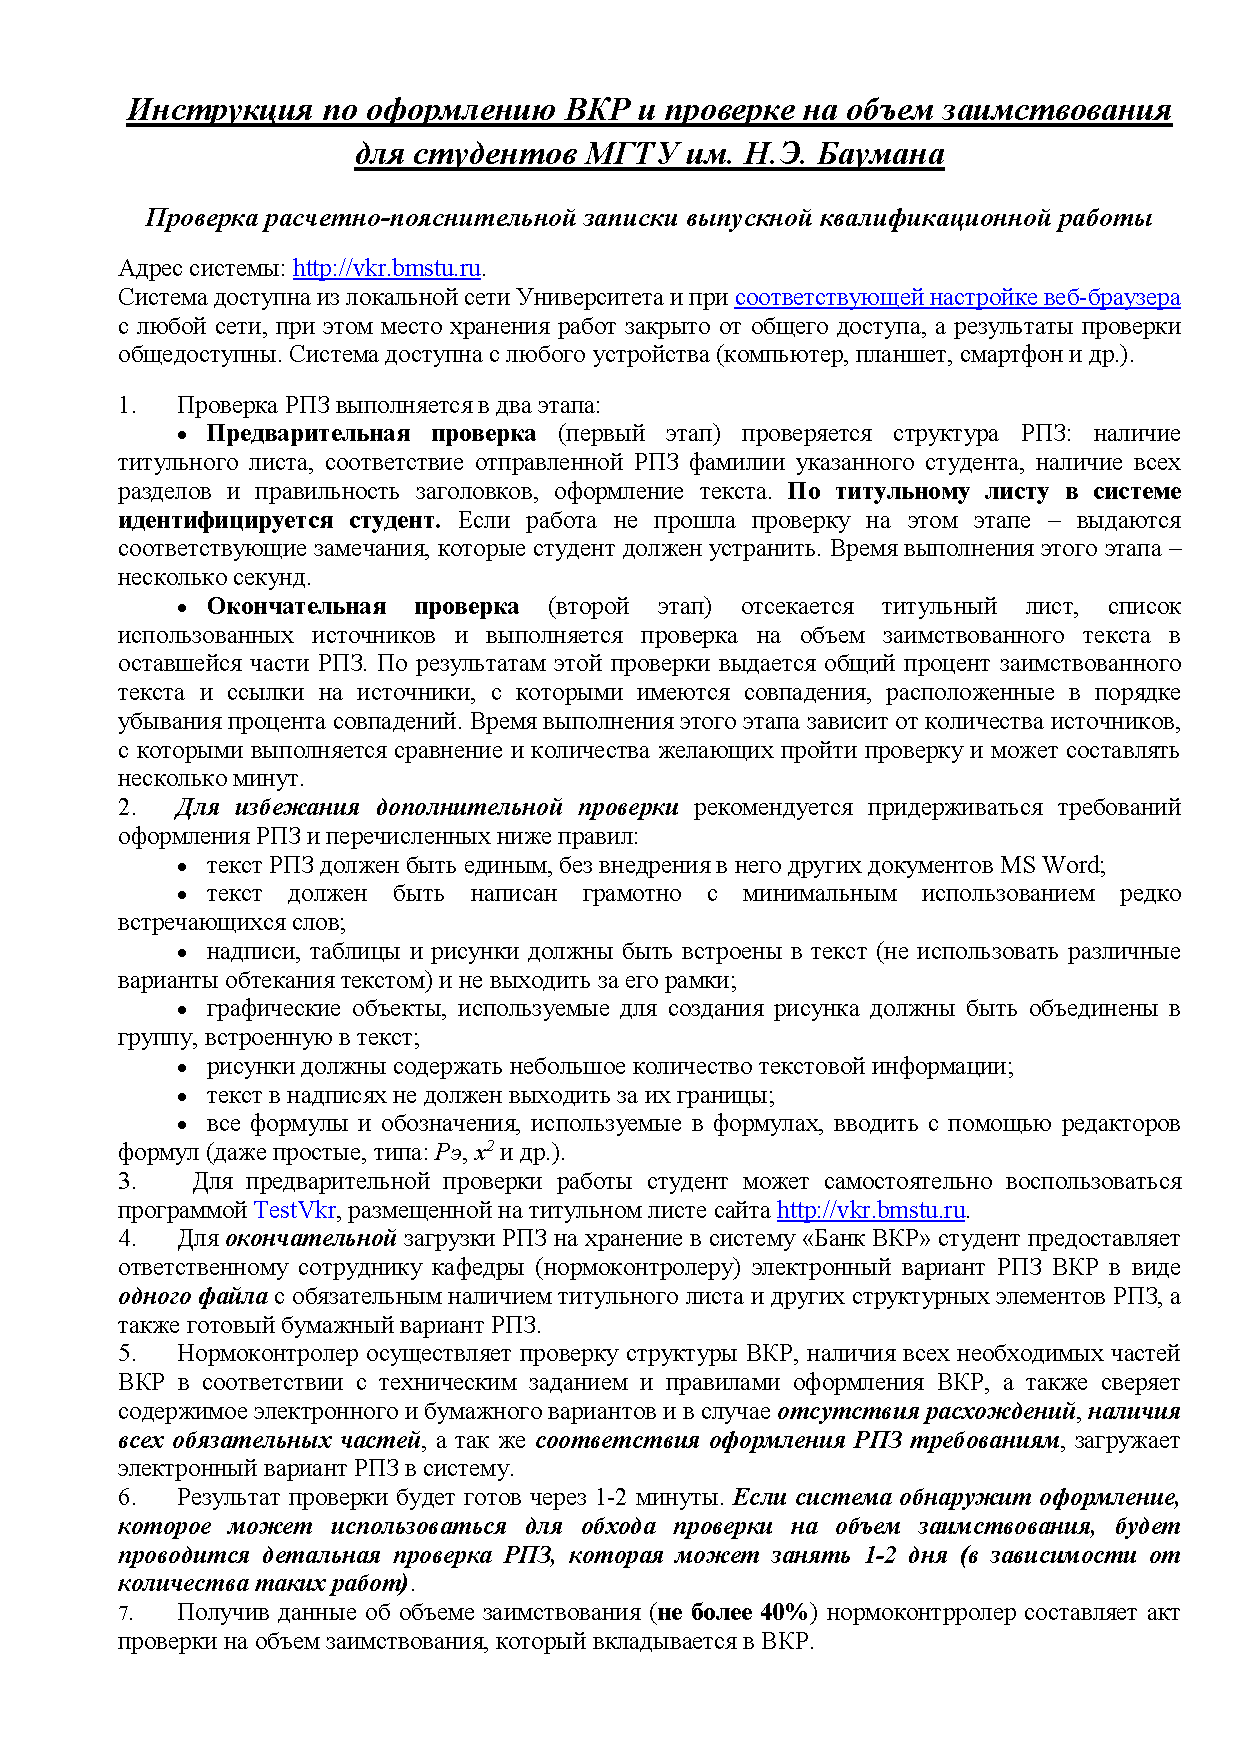
\includepdf[pages=-]{materials/14_05_2023_Памятка_по_оформлению_ВКР_для_студентов_МГТУ_2023.pdf}

%<тут всякие слишком большие ништяки, которые вы хотели бы добавить в отчет>

\ssr{Приложение В}

Памятка <<Как написать для руководителя заготовку задания на дипломную работу>>.

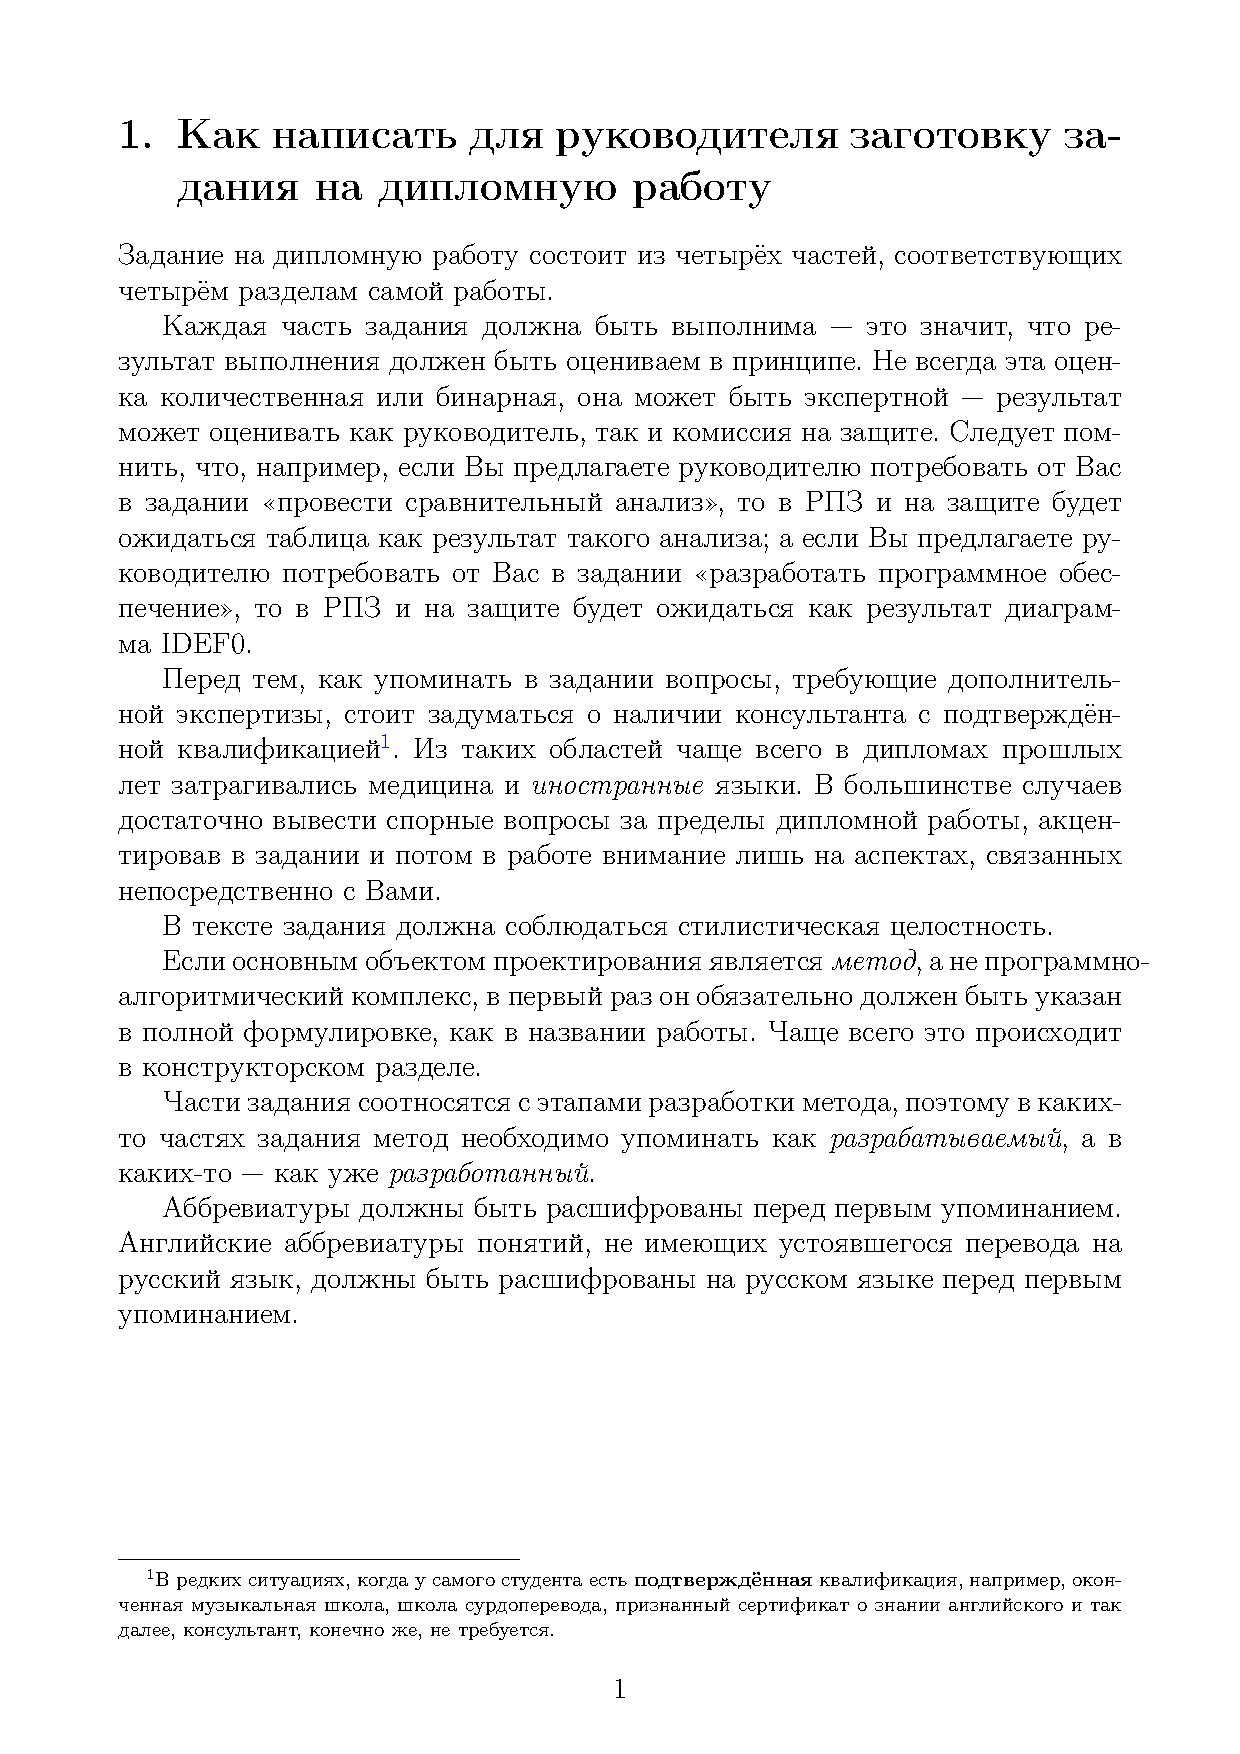
\includepdf[pages=-]{materials/Как_написать_для_руководителя_заготовку_задания_на_дипломную_работу.pdf}

%<тут всякие слишком большие ништяки, которые вы хотели бы добавить в отчет>

\ssr{Приложение Г}

Приложение 1 к положению о нормоконтроле (инструкция по работе с электронно-библиотечной системой <<Банк ВКР>>.

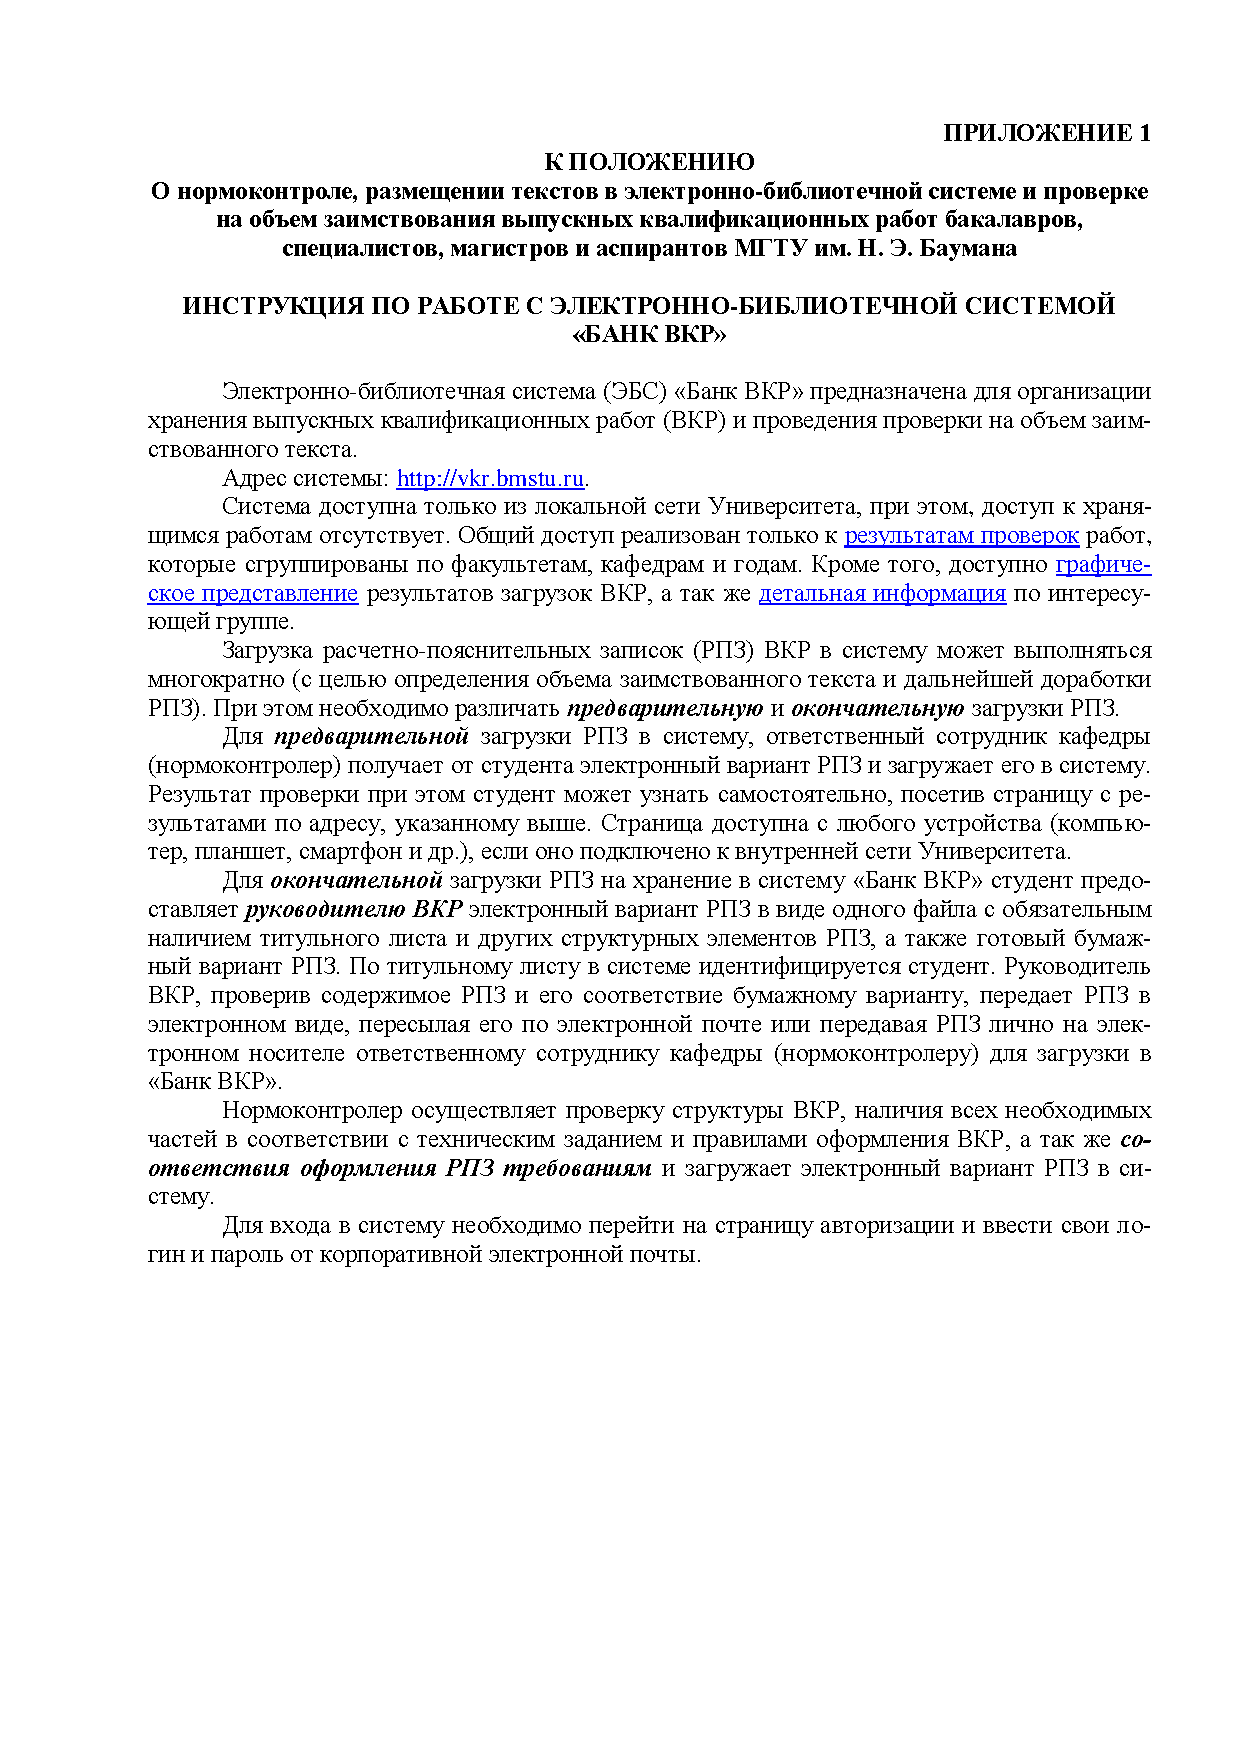
\includepdf[pages=-]{materials/Приложение_1_к_Положению_о_нормоконтроле.pdf}

%<тут всякие слишком большие ништяки, которые вы хотели бы добавить в отчет>

